\documentclass{article}

\usepackage{fancyhdr}
\usepackage{extramarks}
\usepackage{amsmath}
\usepackage{amsthm}
\usepackage{amsfonts}
\usepackage{tikz}
\usepackage[plain]{algorithm}
\usepackage{algpseudocode}
\usepackage[shortlabels]{enumitem}
\usetikzlibrary{automata,positioning}

%
% Basic Document Settings
%

\topmargin=-0.45in
\evensidemargin=0in
\oddsidemargin=0in
\textwidth=6.5in
\textheight=9.0in
\headsep=0.25in

\linespread{1.1}

\pagestyle{fancy}
\lhead{\hmwkAuthorName}
\chead{\hmwkClass\ (\hmwkClassInstructor\ \hmwkClassTime): \hmwkTitle}
\rhead{\firstxmark}
\lfoot{\lastxmark}
\cfoot{\thepage}

\renewcommand\headrulewidth{0.4pt}
\renewcommand\footrulewidth{0.4pt}

\setlength\parindent{0pt}

%
% Create Problem Sections
%

\newcommand{\enterProblemHeader}[1]{
    \nobreak\extramarks{}{Problem \arabic{#1} continued on next page\ldots}\nobreak{}
    \nobreak\extramarks{Problem \arabic{#1} (continued)}{Problem \arabic{#1} continued on next page\ldots}\nobreak{}
}

\newcommand{\exitProblemHeader}[1]{
    \nobreak\extramarks{Problem \arabic{#1} (continued)}{Problem \arabic{#1} continued on next page\ldots}\nobreak{}
    \stepcounter{#1}
    \nobreak\extramarks{Problem \arabic{#1}}{}\nobreak{}
}

\setcounter{secnumdepth}{0}
\newcounter{partCounter}
\newcounter{homeworkProblemCounter}
\setcounter{homeworkProblemCounter}{1}
\nobreak\extramarks{Problem \arabic{homeworkProblemCounter}}{}\nobreak{}

%
% Homework Problem Environment
%
% This environment takes an optional argument. When given, it will adjust the
% problem counter. This is useful for when the problems given for your
% assignment aren't sequential. See the last 3 problems of this template for an
% example.
%
\newenvironment{homeworkProblem}[1][-1]{
    \ifnum#1>0
        \setcounter{homeworkProblemCounter}{#1}
    \fi
    \section{Problem \arabic{homeworkProblemCounter}}
    \setcounter{partCounter}{1}
    \enterProblemHeader{homeworkProblemCounter}
}{
    \exitProblemHeader{homeworkProblemCounter}
}

%
% Homework Details
%   - Title
%   - Due date
%   - Class
%   - Section/Time
%   - Instructor
%   - Author
%

\newcommand{\hmwkTitle}{Homework 4}
\newcommand{\hmwkDueDate}{March 6, 2020}
\newcommand{\hmwkClass}{ENGR 216}
\newcommand{\hmwkClassTime}{Section 509}
\newcommand{\hmwkClassInstructor}{Dr. O}
\newcommand{\hmwkAuthorName}{\textbf{Amari West}}
\newcommand{\hmwkDueTime}{11:55pm \\ 14 Pages}

%
% Title Page
%

\title{
    \vspace{2in}
    \textmd{\textbf{\hmwkClass:\ \hmwkTitle}}\\
    \normalsize\vspace{0.1in}\small{Due\ on\ \hmwkDueDate\ at \hmwkDueTime}\\
    \vspace{0.1in}\large{\textit{\hmwkClassInstructor\ \hmwkClassTime}}
    \vspace{3in}
}

\author{\hmwkAuthorName}
\date{}

\renewcommand{\part}[1]{\textbf{\large Part \Alph{partCounter}}\stepcounter{partCounter}\\}

%
% Various Helper Commands
%

% Useful for algorithms
\newcommand{\alg}[1]{\textsc{\bfseries \footnotesize #1}}

% For derivatives
\newcommand{\deriv}[1]{\frac{\mathrm{d}}{\mathrm{d}x} (#1)}

% For partial derivatives
\newcommand{\pderiv}[2]{\frac{\partial}{\partial #1} (#2)}

% Integral dx
\newcommand{\dx}{\mathrm{d}x}

% Alias for the Solution section header
\newcommand{\solution}{\textbf{\large Solution}}

% Probability commands: Expectation, Variance, Covariance, Bias
\newcommand{\E}{\mathrm{E}}
\newcommand{\Var}{\mathrm{Var}}
\newcommand{\Cov}{\mathrm{Cov}}
\newcommand{\Bias}{\mathrm{Bias}}

% Allow double underline
\def\doubleunderline#1{\underline{\underline{#1}}}

% Allow for units in math mode
\newcommand{\unit}[1]{\ensuremath{\, \mathrm{#1}}}

\begin{document}

\maketitle

\pagebreak

\begin{homeworkProblem}
	A utility pole supports a bundle of wires that apply the 400 N and 650 N forces shown and a guy wire apples the force \textbf{P}.
	\\
	
	\textbf{Part A}
	\\
	
	With $\alpha = 60^{\circ}$, what value \textbf{P} will produce a resultant force that is vertical? Include a diagram.
	\\
	
	\textbf{Part B}
	\\
	
	If the resultant force is to be vertical and \textbf{P} is to be as small as possible, determine the value $\alpha$ should have and the corresponding value of \textbf{P}. Include a diagram.
	\\ 
		
	\underline{\textbf{Given}}
	
	\begin{enumerate}[(i)]
		\item A wire applies a force of 400N in the negative $x$-direction.
		\item A wire applies a force of 650N at $30^{\circ}$ to the horizontal.
		\item For Part A, $\alpha = 60^{\circ}$
	\end{enumerate}
	
	\underline{\textbf{Find}}
	\\
	
	\textbf{Part A}
	\\
	
	The value of \textbf{P} that will produce a vertical resultant force.
	\\
	
	\textbf{Part B}
	\\
	
	The smallest value of \textbf{P} and the value of $\alpha$
	\\ 
	
	\underline{\textbf{Diagram}}
	\\
	
	\textbf{Part A}
	\\
	
	\includegraphics[scale=0.6]{problem1a}
	
	\textbf{Part B}
	\\
	
	\includegraphics[scale=0.6]{problem1b}
	
	\underline{\textbf{Theory}}
	\\
	
	To solve this problem, forces will need to be broken up into their components, and unknown variables must be solved for via systems of equations.
	\\ 
	
	\underline{\textbf{Assumptions}}
	\\
	
	a) The pillar or pole that the point sits on does not create a normal force.
	
	b) The point is in static equilibrium. 
	\\
	
	\underline{\textbf{Solution}}
	\\
	
	Before solving either part, the forces must be broken up into their components and set equivalent to 0.
	
	\[
	\begin{split}
		F_x &= 400\cos{30^{\circ}} + 650 + \boldsymbol{P}\cos{\alpha} = 0
		\\
		F_y &= 400\sin{30^{\circ}} + \boldsymbol{P}\sin{\alpha} = 0
	\end{split}
	\] 
	
	\textbf{Part A}
	\\
	
	Since the resultant force is stated to be vertical, the x-component of the force is equal to zero; therefore, by setting $R_x = 0$ and $\alpha = 60^{\circ}$ the value of $\boldsymbol{P}$ can be found.
	
	\[
	\begin{split}
		0 &= 400\cos{30^{\circ}} - 650 + \boldsymbol{P}\cos{60^{\circ}}
		\\
		0 &= 400\cos{30^{\circ}} - 650 + \boldsymbol{P}\cos{60^{\circ}}
		\\
		-\boldsymbol{P}\cos{60^{\circ}} &= 400\cos{30^{\circ}} - 650
		\\
		\boldsymbol{P} &= \frac{-400\cos{30^{\circ}} + 650}{\cos{60^{\circ}}}
		\\
		\boldsymbol{P} &= -100(4\sqrt{3} - 13)
		\\
		\boldsymbol{P} &= \doubleunderline{607.18}
	\end{split}
	\]
	
	\pagebreak
	
	\textbf{Part B}
	\\
	
	To find the smallest value of \textbf{P}, set $R_x = 0$ and $\alpha = 0$ and use the equation for the net force in the x-direction to solve.
	
	\[
	\begin{split}
		R_x &= 400\cos{30^{\circ} - 650 + \boldsymbol{P}\cos{\alpha}}
		\\
		0 &= 400\cos{30^{\circ}} - 650 + \boldsymbol{P}\cos{\alpha}
		\\
		\boldsymbol{P} &= 650 - 400\cos{30^{\circ}}
		\\
		&= \doubleunderline{303.6}
	\end{split}
	\]
	
	With the new value for \textbf{P}, solve for $\alpha$ as an unknown.
	
	\[
	\begin{split}
		0 &= 400\cos{30^{\circ}} - 650 + 303.6\cos{\alpha}
		\\
		\cos{\alpha} &= \frac{650 - 400\cos{30^{\circ}}}{303.6}
		\\
		\alpha &= \arccos{\left( \frac{650 - 400\cos{30^{\circ}}}{303.6} \right)}
		\\
		&= \doubleunderline{0.4688}
	\end{split}
	\]
	
	\underline{\textbf{Conclusion}}
	\\
	
	\textbf{Part A}
	\\
	
	The value of \textbf{P} that will produce a vertical resultant is \boxed{607.2 \unit{N}}.
	\\
	
	\textbf{Part B}
	\\
	
	The smallest \textbf{P} value is \boxed{303.6 \unit{N}} and the smallest $\alpha$ is \boxed{0.4688 \unit{degrees}.}
	
\end{homeworkProblem}

\pagebreak

\begin{homeworkProblem}
	The system shown below is in equilibrium. Determine the tensions in the cables $AB$ and $BC$ and weight $W_2$. Note that $W_1 = 85$ lbf. FBD is required. 
	\\
	
	
	\underline{\textbf{Given}}
	
	\begin{enumerate}[(i)]
		\item The system is in equilibrium.
		\item $W_1 = 85$ lbf.
	\end{enumerate}
	
	\underline{\textbf{Find}}
	\begin{enumerate}[(i)]
		\item Tension in $AB$.
		\item Tension in $BC$.
		\item Weight of $W_2$.
		\item the value of $\phi$ and $\theta$
	\end{enumerate}
	
	\underline{\textbf{Diagram}}
	\\
	
	\includegraphics[scale=0.9]{problem2a}
	
	\pagebreak
	\textbf{Free-Body}
	
	\includegraphics[scale=0.8]{problem2b}
	
	\underline{\textbf{Theory}}
	\\
	
	To solve this problem, all the forces along the y axis and the x axis must be summed up using Newton's Second Law, and the resulting system of equations must be solved for the unknowns.
	\\
	
	\underline{\textbf{Assumptions}}
	
	\begin{enumerate}[(i)]
		\item The system does not move at either point.
	\end{enumerate}
	
	\underline{\textbf{Solution}}
	\\
	
	Set up the following system of equations based on the free-body diagrams:
	
	\[
	\begin{split}
		\Sigma F_{x} &= |BC|\cos\phi - |AB|\cos\theta = 0
		\\
		\Sigma F_{y} &= |BC|\sin\phi + |AB|\sin\theta - 85 = 0
		\\
		\Sigma F_{y} &= |BC| - W_2 = 0
	\end{split}
	\]
	
	Since the angles are unknown, is trigonometry to find them. \\
	Solve for $\theta$
	
	\[
	\begin{split}
		\arctan \left( \frac{10}{24} \right) &= \theta
		\\
		&= 22.62^{\circ}
	\end{split}
	\]
	
	Solve for $\phi$
	
	\[
	\begin{split}
	\arctan \left( \frac{24}{24} \right) &= \phi
	\\
	&= 45^{\circ}
	\end{split}
	\]
	
	
	
	Use matrices on the calculator to solve for $W_2$, $AB$, and $BC$ to get the solution.
	\\
	
	\underline{\textbf{Conclusion}}
	\\
	
	\begin{itemize}
		\item $W_2 = \doubleunderline{78.86}$
		\item $AB = \doubleunderline{60.41}$
		\item $BC = \doubleunderline{78.86}$
	\end{itemize}
	
\end{homeworkProblem}

\pagebreak

\begin{homeworkProblem}
	The cable-pulley systems shown are used to support a weight $W$.
	Determine the cable tension $T$ in terms of $W$.
	
	Hints:
	\begin{enumerate}[a)]
		\item Draw FBD for point $A$.
		\item Draw FBDs for points $B$ and $C$.
	\end{enumerate}
	
	\underline{\textbf{Given}}
	
	\begin{enumerate}[(i)]
		\item A diagram of the forces acting on the two weights.
	\end{enumerate}	
	
	\underline{\textbf{Find}}

	\begin{enumerate}[(i)]
		\item Draw Free-Body diagrams for each point.
	\end{enumerate}
	
	\underline{\textbf{Diagram}}
	\\
	
	\includegraphics[scale=0.9]{problem3a}
	
	\underline{\textbf{Theory}}
	\\
	
	In order to find all of the forces acting on each point, isolate all the points and draw the forces acting on all of them.
	\\
	
	\underline{\textbf{Assumptions}}
	
	\begin{enumerate}[(i)]
		\item The points are all in static equilibrium. 
	\end{enumerate}
	
	\pagebreak
	
	\underline{\textbf{Solution}}
	\\
	
	\includegraphics[scale=0.8]{problem3b}
	
	\includegraphics[scale=0.8]{problem3c}
	
	\includegraphics[scale=0.8]{problem3d}
	
	\underline{\textbf{Conclusion}}
	\\
	
	The forces above are depicted in the FBD that were drawn.
	
\end{homeworkProblem}

\pagebreak

\begin{homeworkProblem}
	A 50-kg disk is supported by a cable and a wall as shown to the right.
	
	Find the tension in the cable and the force exerted on the disk by the wall (note that for the latter you need to indicate the \underline{direction} of the force, that is report the force using the polar vector representation). FBD is required.
	\\
	
	
	\underline{\textbf{Given}}
	
	\begin{enumerate}[(i)]
		\item The weight of the disk is 50kg.
		\item The angle at which the string and the normal force acts on the disk.
	\end{enumerate}
	
	\underline{\textbf{Find}}
	
	\begin{enumerate}[(i)]
		\item Find the tension for the cable.
		\item Find the normal force. 
	\end{enumerate}
	
	\underline{\textbf{Diagram}}
	\\
	
	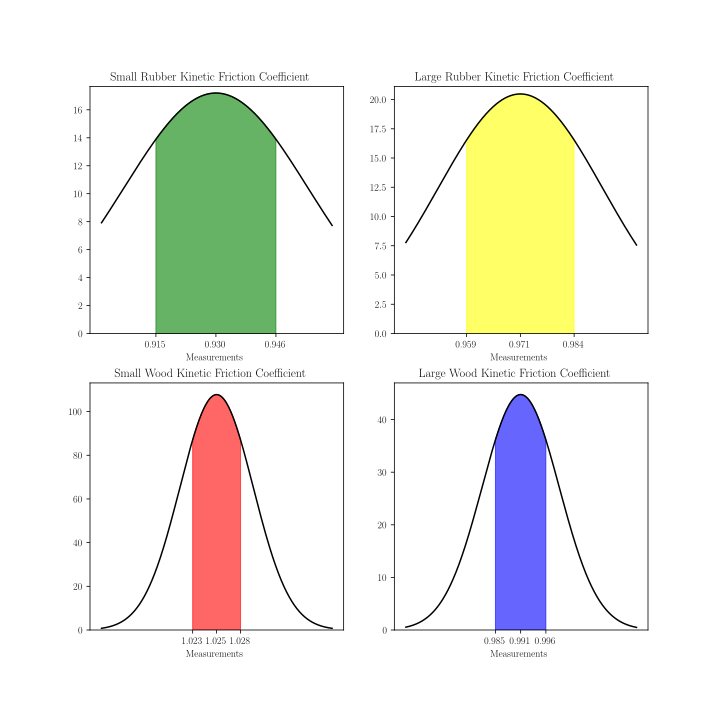
\includegraphics[scale=0.9]{problem4}
	
	\textbf{Free-Body}
	
	\includegraphics[scale=0.9]{problem4b}
	
	\underline{\textbf{Theory}}
	\\
	
	To solve this problem, all the forces along the y axis and the x axis must be summed up using Newton's Second Law, and the resulting system of equations must be solved for the unknowns.
	\\
	
	\underline{\textbf{Assumptions}}
	
	\begin{enumerate}[(i)]
		\item The system is in static equilibrium. 
	\end{enumerate}
	
	\underline{\textbf{Solution}}
	\\
	
	First, the direction of the coordinate plane was reestablished at the angle of the incline of where the disk rests. From there, the angle at which the tension was directed was reestablished to be $20^{\circ}$. After these adjustments were made all the forces were summed up into two equations.
	
	\[
	\begin{split}
		\Sigma F_x &= T\cos20^{\circ} - mg\sin{55^{\circ}}
		\\
		\Sigma F_y &= N + T\sin20^{\circ} - mg\cos55^{\circ}
	\end{split}
	\]
	
	Use matrices to solve for $N$ and $T_1$.
	\\
	
	\underline{\textbf{Conclusion}}
	\\
	
	The following is the solutions for the magnitudes and angles of the forces.
	
	\begin{itemize}
		\item $\doubleunderline{N = 135.1 \angle 90^{\circ}}$
		\item $\doubleunderline{T_1 = 427.6 \angle 20^{\circ}}$
	\end{itemize}
	
\end{homeworkProblem}

\pagebreak

\begin{homeworkProblem}
	Two cables are tied together at C and are loaded as shown.
	\\
	
	\textbf{Part A}
	\\
	
	If $W = 190$ lbf, determine the tension in cable $AC$ and in cable $BC$. FBD is required.
	\\
	
	\textbf{Part B}
	\\
	
	Determine the range of values for $W$ such that the tension will not exceed 240 lbf in either cable.
	\\
	
	\underline{\textbf{Given}}
	\\
	
	\textbf{Part A}
	
	\begin{enumerate}[(i)]
			\item $W = 190$ lbf.
	\end{enumerate}

	\textbf{Part B}
	
	\begin{enumerate}[(i)]
		\item $AB$ nor $BC$ cannot exceed 240 lbf.
	\end{enumerate}
	
	\underline{\textbf{Find}}
	\\
	
	\textbf{Part A}
	
	\begin{enumerate}[(i)]
		\item Tension in $AC$ and tension in $BC$.
	\end{enumerate}
	
	\textbf{Part B}
	
	\begin{enumerate}[(i)]
		\item The range of values for $W$ where neither tension will surpass 240 lbf.
	\end{enumerate}
	
	\underline{\textbf{Diagram}}
	\\
	
	\includegraphics[scale=0.9]{problem5}
	
	\pagebreak
	
	\textbf{Free-Body: Part A @ Point C}
	
	\includegraphics[scale=0.9]{problem5a}
	
	\textbf{Free-Body: Part B @ Point C}
	
	\includegraphics[scale=0.9]{problem5b}
	
	\underline{\textbf{Theory}}
	\\
	
	To solve this problem, all the forces along the y axis and the x axis must be summed up using Newton's Second Law, and the resulting system of equations must be solved for the unknowns.
	\\
	
	\underline{\textbf{Assumptions}}
	
	\begin{enumerate}[(i)]
		\item The system is in static equilibrium. 
	\end{enumerate}
	
	\underline{\textbf{Solution}}
	\\
	
	\textbf{Part A}
	
	Set up the following system of equations based on the free-body diagrams:
	
	\[
	\begin{split}
	\Sigma F_{x} &= |CB|\cos\phi - |AC|\cos\theta - 150\cos\phi = 0
	\\
	\Sigma F_{y} &= |CB|\sin\phi + |AC|\sin\theta - 150\sin\phi - 190 = 0
	\end{split}
	\]
	
	Since the angles are unknown, is trigonometry to find them. \\
	Solve for $\theta$
	
	\[
	\begin{split}
	\arctan \left( \frac{16}{12} \right) &= \theta
	\\
	&= 53.13^{\circ}
	\end{split}
	\]
	
	Solve for $\phi$
	
	\[
	\begin{split}
	\arctan \left( \frac{16}{30} \right) &= \phi
	\\
	&= 28.07^{\circ}
	\end{split}
	\]
	
	Note: $\alpha$ and $\phi$ is the same angle.
	
	
	
	Now, plug in the angles and use matrices on the calculator to solve for $CB$ and $AC$ to get the solution for Part A.
	
	\textbf{Part B}
	
	To solve for the range of values for $W$ in which neither tension will surpass 240 lbf, set $W$ as an unknown and use a guess-and-check method which includes plugging in 240 as the magnitudes for either tension until the smallest value is produced. This method of solving the problem yielded the value of 148.23 lbf for $W$
	\\
	
	\underline{\textbf{Conclusion}}
	\\
	
	\begin{itemize}
		\item $W = \doubleunderline{0 < W < 148.23}$
		\item $AC = \doubleunderline{169.65}$
		\item $CB = \doubleunderline{265.3}$
	\end{itemize}
	
	
\end{homeworkProblem}


\end{document}
